\documentclass{article}
\usepackage[margin=1.5in]{geometry}


\usepackage{blindtext}
\usepackage{graphicx}
\usepackage{wrapfig}
% \usepackage{figure}

\graphicspath{ {./media/} }
\usepackage[square,numbers]{natbib}
\usepackage[nottoc]{tocbibind}
\usepackage{booktabs}
\usepackage{multirow}



\usepackage{tikz}
\usepackage{listings}
\usepackage{setspace}
\definecolor{Code}{rgb}{0,0,0}
\definecolor{Decorators}{rgb}{0.5,0.5,0.5}
\definecolor{Numbers}{rgb}{0.5,0,0}
\definecolor{MatchingBrackets}{rgb}{0.25,0.5,0.5}
\definecolor{Keywords}{rgb}{0,0,1}
\definecolor{self}{rgb}{0,0,0}
\definecolor{Strings}{rgb}{0,0.63,0}
\definecolor{Comments}{rgb}{0,0.63,1}
\definecolor{Backquotes}{rgb}{0,0,0}
\definecolor{Classname}{rgb}{0,0,0}
\definecolor{FunctionName}{rgb}{0,0,0}
\definecolor{Operators}{rgb}{0,0,0}
\definecolor{Background}{rgb}{0.98,0.98,0.98}
\lstdefinelanguage{Python}{
	numbers=left,
	numberstyle=\footnotesize,
	numbersep=1em,
	xleftmargin=1em,
	framextopmargin=2em,
	framexbottommargin=2em,
	showspaces=false,
	showtabs=false,
	showstringspaces=false,
	frame=l,
	tabsize=4,
	% Basic
	basicstyle=\ttfamily\small\setstretch{1},
	backgroundcolor=\color{Background},
	% Comments
	commentstyle=\color{Comments}\slshape,
	% Strings
	stringstyle=\color{Strings},
	morecomment=[s][\color{Strings}]{"""}{"""},
	morecomment=[s][\color{Strings}]{'''}{'''},
	% keywords
	morekeywords={import,from,class,def,for,while,if,is,in,elif,else,not,and,or,print,break,continue,return,True,False,None,access,as,,del,except,exec,finally,global,import,lambda,pass,print,raise,try,assert},
	keywordstyle={\color{Keywords}\bfseries},
	% additional keywords
	morekeywords={[2]@invariant,pylab,numpy,np,scipy},
	keywordstyle={[2]\color{Decorators}\slshape},
	emph={self},
	emphstyle={\color{self}\slshape},
	%
}

\title{\textbf{Proposal for bachelor thesis}\\
Exploration of the influence of graph parameters on the generalization error of Graph Neural Networks}

\author{Author: Wensheng Zhang}

\date{\today}

\begin{document} 

\maketitle

\tableofcontents


\begin{abstract}
The goal of the bachelor thesis is to understand empirically how graph parameters/characteristics influence the generalization error of Graph Neural Networks (GNNs).
\end{abstract}


\section{Setup}
In following, I will descripe training framework, datasets and models for the setup of the experiment.

\subsection{Training Framework}
The training framework is based on PyTorch Geometric~\cite{fey2019fast}. PyTorch Geometric is a library for deep learning on graphs and other irregular structures. It consists of various methods and utilities to ease the implementation of GNNs.

\subsection{Datasets}
The dataset in the experiment is TUDataset~\cite{morris_tudataset_2020}. TUDataset is often used for the GNN evaluation. It consists data across different domains, including small molecules, bioinformatics, social networks and synthetic. Since the size of some datasets are quiet small (under 500 data points/graphs), I use 10-fold cross validation in the training process, in order to fully utilize the data. A dataset is splited into 1:1:8, inwhich one of the folds is treated as test dataset and another is treated as validation dataset. The rest of the folds are used for training. 

\subsection{Models}
I have used GCN layer~\cite{kipf2017semisupervised} and GAT layer~\cite{velickovic2020pointer} in the experiment. In the futher experiment, I will consider to use other GNN layers. In the Appendix, I will provide the code of the example models.


\section{Experiment}
% 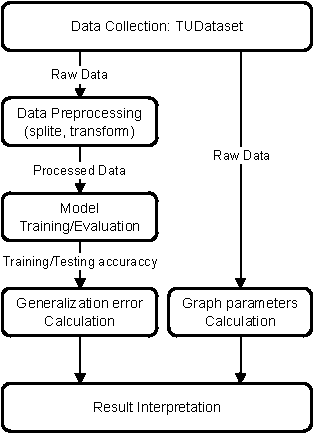
\includegraphics{experiment_procedure.pdf}


\begin{figure}[h]
    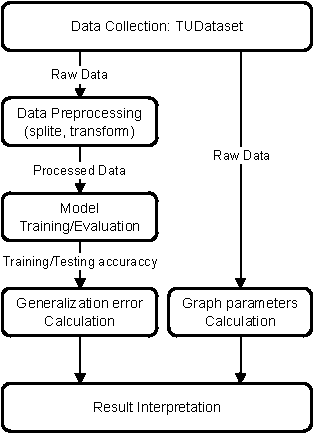
\includegraphics[width=0.5\textwidth]{experiment_procedure.pdf}
    \caption{A illutration of experiment Procedure}
    \label{fig:experiment}
\end{figure}

The experiment consists in three parts: 1. Train the models from datasets and evaluate the models to calculate the generalization error. 2. calculate the parameters of the graphs from the dataset. 3. Analyze the influence of the graph parameters on the generalization error of the GNNs. (See Figure~\ref{fig:experiment})

Here I take seven datasets from TUDataset as examples. The calculated parameters are shown in Table~\ref{tab:parameter}. The generalization error of the models are shown in Table~\ref{tab:error}.


\begin{table}[]
    \centering
    \begin{tabular}{@{}lll@{}}
    \toprule
    \multicolumn{1}{c}{\multirow{2}{*}{Dataset}} & \multicolumn{2}{c}{Parameter}                                            \\ \cmidrule(l){2-3} 
    \multicolumn{1}{c}{}                         & \multicolumn{1}{c}{Ave. degree} & \multicolumn{1}{c}{Ave. shortest path} \\ \midrule
    FRANKENSTEIN                                 & 2.0627         & 3.6521                     \\
    NCI1                                         & 2.1550         & 5.4697                     \\
    COIL-RAG                                     & 1.8277         & 1.0606                     \\
    Letter-high                                  & 1.8896         & 1.5173                     \\
    DD                                           & 4.9790         & 7.9700                     \\
    PTOTEIN\_full                                & 3.7346         & 4.7123                     \\
    COLORS-3                                     & 2.9288         & 2.0945                     \\ \bottomrule
    \end{tabular}
    \caption{The calculated parameters from a set of datasets}
    \label{tab:parameter}
\end{table}

\newpage 

\bibliographystyle{abbrvnat} % or another style like unsrt, alpha, etc.
\bibliography{bibliography} % refers to example.bib

% All reduce Graphs
\newpage 

\section{Appendix} 
 
\subsection*{Example of GCN model}

\begin{lstlisting}[language=Python]
import torch
from torch import nn
import torch.nn.functional as F
from torch_geometric.nn import GCNConv
from torch_geometric.nn import global_mean_pool


class GCN(torch.nn.Module):
    def __init__(self, in_channels, hidden_channels, out_channels):
        super().__init__()
        self.conv1 = GCNConv(in_channels, hidden_channels)
        self.conv2 = GCNConv(hidden_channels, hidden_channels)
        self.conv3 = GCNConv(hidden_channels, hidden_channels)
        self.conv4 = GCNConv(hidden_channels, hidden_channels)
        self.conv5 = GCNConv(hidden_channels, hidden_channels)
        self.fc1 = nn.Linear(hidden_channels, hidden_channels)
        self.fc2 = nn.Linear(hidden_channels, out_channels)


    def forward(self, x, edge_index, batch, edge_weight=None):
        x = self.conv1(x, edge_index, edge_weight).relu()
        x = self.conv2(x, edge_index, edge_weight).relu()
        x = self.conv3(x, edge_index, edge_weight).relu()
        x = self.conv4(x, edge_index, edge_weight).relu()
        x = self.conv5(x, edge_index, edge_weight).relu()
        x = global_mean_pool(x, batch)
        x = self.fc1(x).relu()
        x = F.dropout(x, p=0.5, training=self.training)
        x = self.fc2(x)
        return x
    
    def reset_parameters(self):
        for (_, module) in self._modules.items():
            module.reset_parameters()

\end{lstlisting}

\end{document}